\section{Scope of the ESMF}
\label{sec:shortscope}

The ESMF includes
\begin{itemize}
\item services and standards for coupling high-level model components; and 
\item an infrastructure of general utilities for composing model components.
\end{itemize}  
The model components we will support initially are those included in the ESMF {\it Joint 
Milestone Codeset (JMC)}, which consists of fifteen climate, weather and data 
assimilation applications.
These codes, developed by ESMF investigators and their colleagues, include the National 
Centers for Environmental Prediction (NCEP) Forecast 
Suite \cite{parrish, derber1}, applications running under the Geophysical Fluid Dynamics
Laboratory (GDFL) Flexible Modeling System (FMS) \cite{fms}, applications running under 
the Goddard Earth Modeling System {GEMS} \cite{gems}, the Community Climate System 
Model (CCSM) \cite{ccsm}, the Weather Research and Forecast Model (WRF) \cite{wrf}, and 
more.  A full listing of JMC codes is available on the ESMF website, 
\htmladdnormallink{http://www.esmf.ucar.edu}{http://www.esmf.ucar.edu},
via the {\bf Applications} link on the navigation bar.  

Components of the JMC applications include regional and global atmospheres, regional and 
global oceans, land models, sea ice models, and data assimilation systems.  Components will 
recode or wrap their internal data structures in order to provide a standard ESMF interface 
and employ ESMF intercomponent communications.  The ESMF coupling services will include 
software for representing data distributions, interpolating and redistributing gridded data, 
and load balancing computations.

Coupling services will be built upon a base of general data structures and utilities.
Data structures and associated methods are defined for common constructs such as 
fields and grids.  
Supporting the coupling services and accessible to model developers are a set of 
general ESMF utilities.  These include error handling, timing and profiling, 
message logging, low-level I/O and communication, time management, and parameter 
specification.

\begin{figure}
\scalebox{0.7}{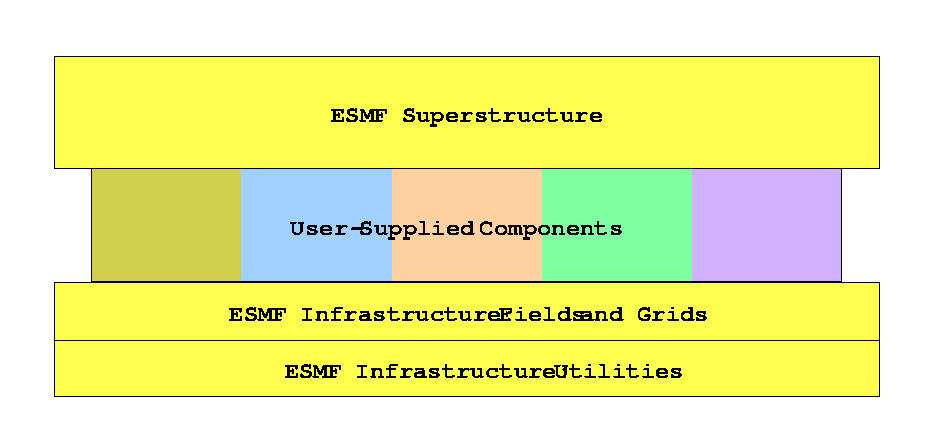
\includegraphics{Sandwich.eps}}
\caption[{ESMF Architecture}] {The simplest view of the ESMF architecture
is that it consists of an infrastructure for developing components and 
a superstructure for assembling applications.}
\label{fig:sandwich}
\end{figure}







